\documentclass{beamer}
\usetheme{Berlin}
\usepackage{graphicx}
\usepackage[UKenglish]{isodate}
\usepackage{tikz}

\graphicspath{{./images/}}
\beamertemplatenavigationsymbolsempty

\title{Processor Simulator}
\author{George Herbert}
% \institute[University of Bristol, Bristol, U.K.]{University of Bristol\\Bristol, U.K.}
\date{\today}

\begin{document}

\begin{frame}
    \titlepage
\end{frame}

\section{Architecture}
\begin{frame}{High-Level Architecture Diagram}
    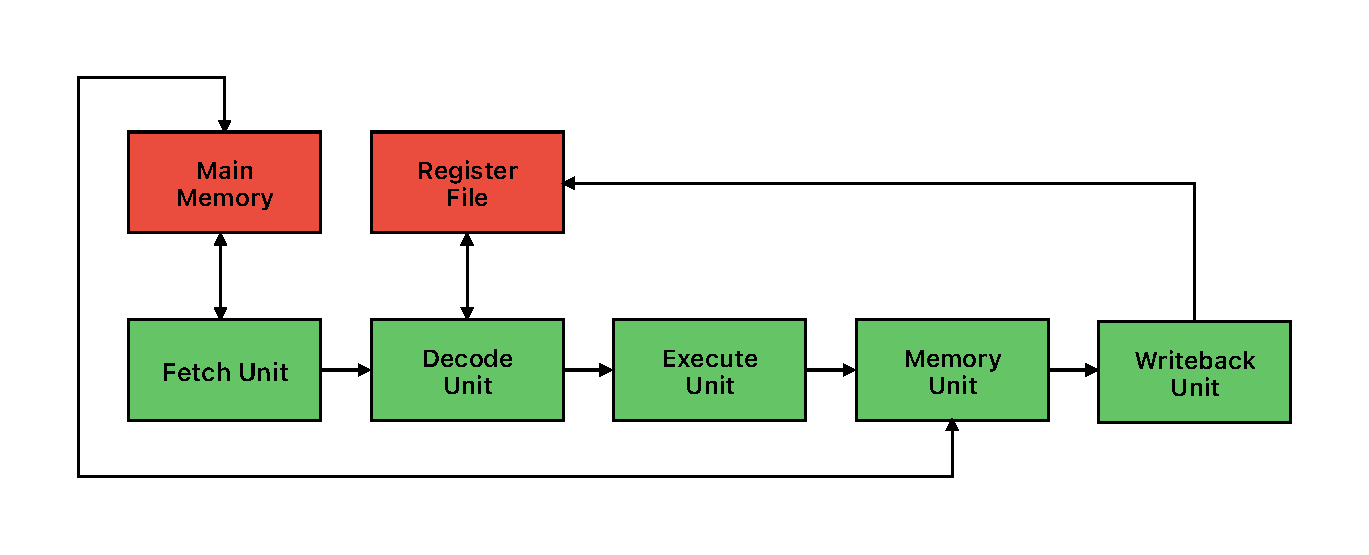
\includegraphics[width = \textwidth]{architecture.pdf}
\end{frame}

\begin{frame}{Features}
    \begin{itemize}
        \item Non-pipelined and scalar
        \item Five-stages: fetch, decode, execute, memory, writeback
        \item Implements the RV32I base integer instruction set, except for the FENCE, ECALL, and EBREAK instructions
        \item Operation of each unit is dictated by control signals produced by the decode unit
    \end{itemize}
\end{frame}

\section{Benchmarks}
\begin{frame}{Benchmark Kernels Overview}
    \begin{itemize}
        \item\textbf{Factorial}: Computes $12!$ with multiplication implemented via repeated addition.
        \item\textbf{Bubble Sort}: Sorts a descending list of $1000$ integers into ascending order using the bubble sort algorithm.
        \item\textbf{Euclidean}: Computes the greatest common divisor of $7^3\cdot17^5$ and $7^3\cdot2$ using Euclid's original subtraction-based algorithm.
        \item\textbf{Matrix Multiply}: Multiplies a $10\times50$ matrix by a $50\times10$ matrix, with multiplication again implemented via repeated addition.
    \end{itemize}
\end{frame}

\begin{frame}{Benchmark Results}
    \begin{table}[]
        \begin{center}
        \begin{tabular}{l|cc|c}
        \textbf{Kernel}&\textbf{Instructions}&\textbf{Cycles}&\textbf{IPC}\\
        \hline\hline
        Factorial&439,547,610&2,197,738,050&0.2\\
        \hline
        Bubble Sort&22,508,527&112,542,635&0.2\\
        \hline
        Euclidean&7,809,251&39,046,255&0.2\\
        \hline
        Matrix Multiply&16,571,974&82,859,870&0.2\\
        \end{tabular}
        \end{center}
    \end{table}
\end{frame}

\section{Future Work}

\begin{frame}{Plans for the Final Submission}
    The following is a list of features that I would ideally like to implement for the final submission:
    \begin{itemize}
        \item Pipelining
        \item Out-of-order execution via Tomasulo's algorithm
        \item Multiple execution units
        \item Branch prediction
        \item Speculative execution
        \item More benchmark kernels
    \end{itemize}
\end{frame}


\end{document}
